\Variant{23.02.2025 (2-smena)}
\QQ{1}{Agar $a$, $b$ raqamlar uçun $5a+\dfrac5{11}b=45$ tenglik örinli bölsa, $2a+b$ ni toping.
\Opts{$16$}{$18$}{$12$}{$24$}}
\QQ{2}{Agar
\[x=1+4+7+\dots+301,\qquad y=2+8+14+\dots+602\]
bölsa, $\dfrac yx$ ni hisoblang.
\Opts{$2$}{$2023$}{$2022$}{$2021$}}
\QQ{3}{Basseynda $4$ ta quvur bor. Birinçi va ikkinçi quvur basseynni töldiradi. Uçinçi va törtinçi quvur basseynni böşatadi. $4$ ta quvur birdaniga oçilsa basseyn $5$ soatda töladi. Faqat birinçi, ikkinçi va uçinçi quvurlar oçilsa $3$ soatda töladi. Faqat birinçi, uçinçi va törtinçi quvurlar oçilsa $30$ soatda töladi. Faqat birinçi va uçinçi quvurlar oçilsa basseyn neça soatda töladi?
\Opts{$10$ soat}{$4$ soat}{$6$ soat}{$5$ soat}}
\QQ{4}{Meva tarkibida $80\%$ suv bor. Quritilgandan keyin $25$ kg kamayib, suvi $60\%$ bölib qoldi. Dastlab meva neça kg bölgan?
\Opts{$60$}{$70$}{$50$}{$40$}}
\QQ{5}{Ifodaning qiymatini toping:
\[\frac{3^9\cdot3^{-6}\cdot5^4+625\cdot27\cdot\left(\frac15\right)^{-1}}{2\cdot3^2\cdot5^2-4\cdot9\cdot\left(\frac25\right)^{-2}}\]
\Opts{$150$}{$100$}{$450$}{$125$}}
\QQ{6}{Agar $a=7-\sqrt3$ ga teng bölsa, $a^2-14a+51$ ning qiymatini toping.
\Opts{$4$}{$5$}{$6$}{$3$}}
\QQ{7}{Ifodani soddalaştiring:
\[\frac{\left(\sqrt3-\sqrt[4]{45}\right)^2}{1-2\sqrt[4]5+\sqrt5}\]
\Opts{$1$}{$\sqrt3$}{$2$}{$3$}}
\QQ{8}{Arifmetik progressiyada $a_4+a_7+a_9+a_{11}+a_{14}=45$ bölsa, dastlabki ön yettita hadi yiğindisini toping.
\Opts{$153$}{$85$}{$255$}{$765$}}
\QQ{9}{Geometrik progressiyada $S_4=80$ va $S_8=6560$ ga teng bölsa, $S_6$ ni toping.
\Opts{$2540$}{$2320$}{$728$}{$2640$}}
\QQ{10}{Agar $|c|<|b|<|a|$ va $a<0$, $b>0$, $c<0$ bölsa, $\dfrac{a|b-c|}{|a|}+\dfrac{b|c-a|}{|b|}+\dfrac{c|a-b|}{|c|}$ ni hisoblang.
\Opts{$2a-2b$}{$0$}{$2c-2a$}{$2c-2b$}}
\QQ{11}{Ifodani soddalaştiring:
\[\frac{a^4-64}{a^2+8}-\frac{a^6-512}{a^4+8a^2+64}\]
\Opts{$2\left(a^2-8\right)$}{$16$}{$0$}{$2\left(a^2+8\right)$}}
\QQ{12}{Quyidagi tenglamaning $\left[\dfrac\pi2;\,\dfrac{17\pi}2\right]$ oraliqda neçta yeçimi bor?
\[\cos2x-1=5\sin x+2\]
\Opts{$7$}{$6$}{$8$}{$5$}}
\QQ{13}{Ifodani soddalaştiring:
\[\frac{\sin\alpha}{\tg\left(\frac\pi4-\frac\alpha2\right)(1+\sin\alpha)}\]
\Opts{$\tg\alpha$}{$\ctg\alpha$}{$-\tg\alpha$}{$-\ctg\alpha$}}
\QQ{14}{Tengsizlikni yeçing:
\[x^2\cdot3^x+9>3^x+9\cdot x^2\]
\Opts{$(-\infty;\,-1)\cup(1;\,2)$}{$(-1;\,\infty)$}{$(-1;\,1)\cup(2;\,\infty)$}{$(-1;\,2)$}}
\QQ{15}{$\log_{0,5}\log_3\log_2\dfrac{x^3+8x}{x-5}\le0$ tengsizlikning eng kiçik natural yeçimini toping.
\Opts{$9$}{$8$}{$7$}{$6$}}
\QQ{16}{Tengsizlikning natural yeçimlari yiğindisini toping:
\[245x-x^6>0\]
\Opts{$5$}{$3$}{$6$}{$7$}}
\QQ{17}{Quyidagi tenglamalar sistemasi neçta yeçimga ega?
\[\begin{cases}x^2=4x+5y\\ y^2=5x+4y\end{cases}\]
\Opts{$1$}{$2$}{$3$}{$4$}}
\QQ{18}{Rasmda berilgan maʼlumotlar asosida $a$, $b$, $c$ larni taqqoslang.
\qfig{\begin{tikzpicture}[scale=0.9,font=\small]
\draw[-{Stealth[length=4pt]}] (-1.8,0)--(2.1,0) node[right] {$x$}; \draw[-{Stealth[length=4pt]}] (0,-0.4)--(0,3.2) node[left] {$y$};
\draw[thick,domain=-0.75:0.75,samples=40] plot (\x,{5*\x*\x}); \draw[thick,domain=-1.1:1.1,samples=40] plot (\x,{2.4*\x*\x}); \draw[thick,domain=-1.55:1.55,samples=40] plot (\x,{1.2*\x*\x});
\node[right,rotate=75] at (0.72,2.85) {\scriptsize$y=bx^2$}; \node[right,rotate=75] at (1.1,2.95) {\scriptsize$y=ax^2$}; \node[right,rotate=75] at (1.56,2.95) {\scriptsize$y=cx^2$};
\end{tikzpicture}}
\Opts{$a>b>c$}{$b>a>c$}{$c>a>b$}{$b>c>a$}}
\QQ{19}{Tengsizlikning butun yeçimlari yiğindisini toping:
\[\left(x^2-5x+10\right)\left(x^2-5x+12\right)<48\]
\Opts{$10$}{$7$}{$6$}{$5$}}
\QQ{20}{Agar $x_1$ va $x_2$ sonlari $2x^2+9x+5=0$ tenglamaning ildizlari bölsa, $\dfrac1{x_1^2}+\dfrac1{x_2^2}$ ni hisoblang.
\Opts{$\dfrac{53}{25}$}{$\dfrac{49}{25}$}{$\dfrac{61}{25}$}{$\dfrac{13}{25}$}}
\QQ{21}{Neçta natural son $f(x)=6\sin x-4\cos x$ funksiyaning qiymatlar sohasiga tegişli?
\Opts{$15$}{$7$}{$4$}{$14$}}
\QQ{22}{Aniq integralni hisoblang:
\[\int_2^4\frac3{5-4x-x^2}\,dx\]
\Opts{$\ln\dfrac37$}{$\ln\sqrt{\dfrac37}$}{$\ln\sqrt{\dfrac73}$}{$\ln\dfrac73$}}
\QQ{23}{Agar $f(x)=\dfrac{2^{2x}}{\sqrt{2-2^{2x}}}$ ga teng bölsa, $f'(0)$ ni toping.
\Opts{$\dfrac32\ln2$}{$\dfrac32\ln4$}{$\dfrac32\ln8$}{$\dfrac32\ln16$}}
\QQ{24}{Ikkita aylana taşqi ravişda urinadi. Ularning diametrlari $10$ dm va $18$ dm ga teng bölsa, aylanalar markazlari orasidagi masofani toping.
\qfig{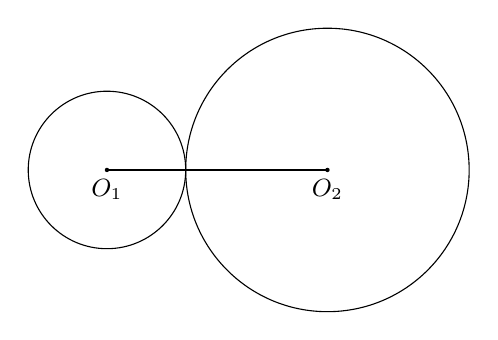
\begin{tikzpicture}[scale=0.2,font=\small]
\coordinate (O1) at (0,0); \coordinate (O2) at (14,0);
\draw (O1) circle (5); \draw (O2) circle (9); \draw (O1)--(O2); \fill (O1) circle (4pt); \fill (O2) circle (4pt);
\node[below] at (O1) {$O_1$}; \node[below] at (O2) {$O_2$};
\end{tikzpicture}}
\Opts{$8$}{$28$}{$14$}{$20$}}
\QQ{25}{Teng yonli uçburçakning uçidagi burçagi $30^\circ$ ga teng. Asosidan olingan $E$ nuqtadan yon tomonlarigaça bölgan eng qisqa masofalar $3$ va $9$ ga teng. Uçburçak yuzini toping.
\qfig{\begin{tikzpicture}[scale=0.22,font=\small]
\coordinate (B) at (0,0); \coordinate (C) at (12.42,0); \coordinate (A) at (6.21,23.18); \coordinate (E) at (3.106,0);
\coordinate (P) at ($(A)!(E)!(B)$); \coordinate (Q) at ($(A)!(E)!(C)$);
\draw (A)--(B)--(C)--cycle; \draw (E)--(P); \draw (E)--(Q);
\node[below left] at (B) {$B$}; \node[below right] at (C) {$C$}; \node[above] at (A) {$A$}; \node[below] at (E) {$E$};
\node[below] at (6.21,20.4) {\scriptsize$30^\circ$};
\end{tikzpicture}}
\Opts{$144$}{$108$}{$36\left(2+\sqrt3\right)$}{$36\left(2-\sqrt3\right)$}}
\QQ{26}{$ABC$ töğri burçakli uçburçak gipotenuzasi uzunligi $15$ ga, $\sin\angle ACB=0{,}6$ ga teng bölsa, uçburçak yuzini toping.
\qfig{\begin{tikzpicture}[scale=0.3,font=\small]
\coordinate (A) at (0,0); \coordinate (C) at (12,0); \coordinate (B) at (0,9);
\draw (A)--(B)--(C)--cycle; \draw (0,0.7)--(0.7,0.7)--(0.7,0);
\draw (C)+(143.13:1.5) arc (143.13:180:1.5);
\node[below left] at (A) {$A$}; \node[above left] at (B) {$B$}; \node[below right] at (C) {$C$};
\node[above right] at (6,4.5) {$15$}; \node at (9.6,0.5) {\scriptsize$\alpha$};
\end{tikzpicture}}
\Opts{$56$}{$54$}{$108$}{$36$}}
\QQ{27}{Ikkita bir xil kvadrat ustma-ust qöyilib, biri ikkinçisi ustida $45^\circ$ ga burildi. Böyalgan soha yuzining $ABCD$ kvadrat yuziga nisbatini toping.
\qfig{\begin{tikzpicture}[scale=1.15,font=\small]
\coordinate (A) at (-1,-1); \coordinate (B) at (-1,1); \coordinate (C) at (1,1); \coordinate (D) at (1,-1);
\coordinate (E) at (0,-1.414); \coordinate (F) at (-1.414,0); \coordinate (G) at (0,1.414); \coordinate (H) at (1.414,0);
\fill[qfill] (G)--(-0.414,1)--(0.414,1)--cycle; \fill[qfill] (H)--(1,0.414)--(1,-0.414)--cycle; \fill[qfill] (E)--(-0.414,-1)--(0.414,-1)--cycle; \fill[qfill] (F)--(-1,0.414)--(-1,-0.414)--cycle;
\draw (A)--(B)--(C)--(D)--cycle; \draw (E)--(F)--(G)--(H)--cycle;
\node[below left] at (A) {$A$}; \node[above left] at (B) {$B$}; \node[above right] at (C) {$C$}; \node[below right] at (D) {$D$};
\node[below] at (E) {$E$}; \node[left] at (F) {$F$}; \node[above] at (G) {$G$}; \node[right] at (H) {$H$};
\end{tikzpicture}}
\Opts{$\dfrac12$}{$3+2\sqrt2$}{$3-2\sqrt2$}{$\sqrt2-1$}}
\QQ{28}{Muntazam köpburçakning tomoni $2\sqrt3$ ga va içki çizilgan aylana radiusi $3$ ga teng bölsa, köpburçak yuzini toping.
\Opts{$18\sqrt3$}{$12\sqrt3$}{$24\sqrt3$}{$20\sqrt3$}}
\QQ{29}{Rasmda qirrasi uzunligi $3$ ga teng bölgan $ABCDA_1B_1C_1D_1$ kub tasvirlangan. Şunga köra $\left(\overrightarrow{AD}+\overrightarrow{DC}\right)\cdot\left(\overrightarrow{CC_1}+\overrightarrow{C_1D_1}\right)$ ni hisoblang.
\qfig{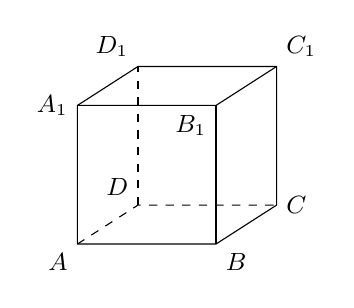
\begin{tikzpicture}[scale=1.1,font=\small]
\coordinate (A) at (0,0); \coordinate (B) at (1.6,0); \coordinate (C) at (2.3,0.45); \coordinate (D) at (0.7,0.45);
\coordinate (A1) at (0,1.6); \coordinate (B1) at (1.6,1.6); \coordinate (C1) at (2.3,2.05); \coordinate (D1) at (0.7,2.05);
\draw (A)--(B)--(C)--(C1)--(D1)--(A1)--cycle; \draw (A1)--(B1)--(C1); \draw (B)--(B1);
\draw[dashed] (A)--(D)--(C); \draw[dashed] (D)--(D1);
\node[below left] at (A) {$A$}; \node[below right] at (B) {$B$}; \node[right] at (C) {$C$}; \node[above left] at (D) {$D$};
\node[left] at (A1) {$A_1$}; \node[below left] at (B1) {$B_1$}; \node[above right] at (C1) {$C_1$}; \node[above left] at (D1) {$D_1$};
\end{tikzpicture}}
\Opts{$3$}{$9$}{$-9$}{$-3$}}
\QQ{30}{$ABCD$ töğri törtburçak tekisligiga $S$ nuqtadan $SA$ perpendikulyar tuşirildi. $SB=6$, $SC=9$ va $SD=7$ bölsa, $SA$ ni toping.
\Opts{$1$}{$3$}{$2$}{$4$}}
\QQ{31}{$A=\{24$ ning natural böluvçilari$\}$, $B=\{16$ ning natural böluvçilari$\}$, $C=\{20$ ning natural böluvçilari$\}$ bölsa, $n(A)+n(B)-n(C)$ ni hisoblang. (Bu yerda $n(A)$ — $A$ töplamning elementlari soni.)
\Opts{$9$}{$7$}{$3$}{$8$}}
\QQ{32}{$3$, $5$, $7$ raqamlaridan foydalanib $10^5$ dan kiçik neçta natural son tuziş mumkin?
\Opts{$363$}{$243$}{$729$}{$512$}}
\QQ{33}{\Moslash{Prizma va silindr hajmlari teng. Prizmaning asosi trapetsiyadan iborat. Trapetsiyaning kiçik asosi trapetsiyaning balandligiga teng, kiçik asosi katta asosidan $2$ marta kiçik. ($\pi=3$ deb oling.)
\par\centering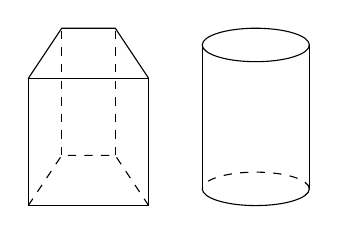
\begin{tikzpicture}[scale=0.85,font=\small]
\draw (0,0)--(1.8,0)--(1.8,1.9)--(0,1.9)--cycle; \draw (0,1.9)--(0.5,2.65)--(1.3,2.65)--(1.8,1.9);
\draw[dashed] (0,0)--(0.5,0.75)--(1.3,0.75)--(1.8,0); \draw[dashed] (0.5,0.75)--(0.5,2.65); \draw[dashed] (1.3,0.75)--(1.3,2.65);
\draw (2.6,0.25)--(2.6,2.4); \draw (4.2,0.25)--(4.2,2.4); \draw (3.4,2.4) ellipse (0.8 and 0.25);
\draw (2.6,0.25) arc (180:360:0.8 and 0.25); \draw[dashed] (4.2,0.25) arc (0:180:0.8 and 0.25);
\end{tikzpicture}}{A) $\sqrt3$\par B) $\sqrt2$\par C) $3$\par D) $4$\par E) $5$\par F) $2$}{Prizmaning balandligi bilan silindrning balandligi teng. Trapetsiyaning kiçik asosi silindr radiusidan neça marta katta?}{Trapetsiyaning kiçik asosi silindr radiusidan $2$ marta katta. Silindr balandligining prizma balandligiga nisbatini toping.}{Trapetsiyaning kiçik asosi silindr radiusidan $2$ marta katta. Prizma asosining yuzi $6$ ga teng. Silindr asosining yuzini toping.}}
\QQ{36}{Tenglamalar sistemasini yeçing:
\[\begin{cases}\dfrac4{x+y}+\dfrac4{x-y}=3\\[2mm] (x+y)^2+(x-y)^2=20\end{cases}\]
\AB{Tenglamalar sistemasining neçta juft $(x;\,y)$ yeçimi bor?}{Agar tenglamaning yeçimlari $(x_1;\,y_1)$, $(x_2;\,y_2)$, \dots, $(x_n;\,y_n)$ bölsa, $x_1+x_2+\dots+x_n$ ni toping.}}
\QQ{37}{Tenglamani yeçing:
\[\left|\cos\left(\frac{2\pi}3\sin\frac{2x}3\right)+1\right|=\frac12\]
\AB{Tenglamaning $[-\pi;\,4\pi]$ oraliqdagi ildizlar sonini toping.}{Tenglamaning $[-\pi;\,4\pi]$ oraliqdagi ildizlari yiğindisini toping.}}
\QQ{38}{Rasmda uçlari $y_1$ va $y_2$ funksiyalarda bölgan eng katta yuzali $ABCD$ töğri törtburçak tasvirlangan.
\qfig{\begin{tikzpicture}[x=0.75cm,y=0.42cm,font=\small]
\draw[-{Stealth[length=4pt]}] (-2.4,0)--(2.9,0) node[right] {$x$}; \draw[-{Stealth[length=4pt]}] (0,-0.5)--(0,7.6) node[left] {$y$};
\fill[qfill] (-1.155,3.333) rectangle (1.155,6);
\draw[thick,domain=-2.1:2.1,samples=50] plot (\x,{\x*\x+2}); \draw (-2.3,6)--(2.6,6);
\draw (-1.155,3.333) rectangle (1.155,6); \fill (0,2) circle (1.5pt);
\node[above left] at (-1.155,6) {$A$}; \node[above right] at (1.155,6) {$B$}; \node[below right] at (1.155,3.333) {$C$}; \node[below left] at (-1.155,3.333) {$D$};
\node[below right] at (0,2) {$(0;\,2)$}; \node[right] at (2.6,6) {$y_2=6$}; \node[right] at (1.75,4.6) {$y_1=x^2+2$};
\end{tikzpicture}}
\AB{$ABCD$ töğri törtburçak yuzini toping.}{$AC$ diagonal uzunligini toping.}}
\QQ{39}{$f(x)$ funksiya uçun
\[(x+1)f(x)+f\left(\frac1x\right)=\frac{4x+2}{x+1}\]
bölsin.
\AB{$f(2)$ ni toping.}{$f^2(3)$ ni toping.}}
\QQ{40}{Rasmda $y_1$ — töğri çiziq, $y_2$ — parabola va $x=1$ simmetriya öqi berilgan bölsa, rasmda berilgan maʼlumotlar asosida:
\qfig{\begin{tikzpicture}[x=0.55cm,y=0.33cm,font=\small]
\fill[qfill] (0,2) -- plot[domain=0:3,samples=30] (\x,{-\x*\x+2*\x+8}) -- (3,5) -- cycle;
\draw[-{Stealth[length=4pt]}] (-3.2,0)--(5.6,0) node[right] {$x$}; \draw[-{Stealth[length=4pt]}] (0,-1.5)--(0,10.6) node[left] {$y$};
\draw[thick,domain=-2.6:4.5,samples=60] plot (\x,{-\x*\x+2*\x+8}); \draw[thick] (-2.8,-0.8)--(4.6,6.6);
\draw[dashed] (1,-1.5)--(1,10.2); \draw (0,2)--(0,8);
\fill (0,8) circle (2pt); \fill (0,2) circle (2pt); \fill (-2,0) circle (2pt); \fill (3,5) circle (2pt);
\node[left] at (0,8) {$(0;\,8)$}; \node[below right] at (0,2) {$(0;\,2)$}; \node[above left] at (-2,0) {$A(-2;\,0)$}; \node[right] at (3.05,5) {$B(x;\,y)$};
\node[below right] at (1,0) {$x=1$}; \node[above] at (4.6,6.6) {$y_1$}; \node[right] at (4.2,1.5) {$y_2$};
\end{tikzpicture}}
\AB{$x+y$ ni hisoblang.}{Böyalgan soha yuzini toping.}}
\QQ{41}{$ABC$ uçburçakning $A$ uçidan $AH$ balandlik tuşirilgan. $ABH$ va $AHC$ uçburçaklarga içki aylanalar çizilgan bölib, bunda $M$ va $O$ nuqtalar $ABH$ uçburçakka içki çizilgan aylananing mos ravişda $BH$ va $AH$ tomonlariga urinuvçi nuqtalari, $T$ va $N$ nuqtalar $AHC$ uçburçakka içki çizilgan aylananing mos ravişda $AH$ va $HC$ tomonlariga urinuvçi nuqtalari. $MO$ töğri çiziq $NT$ kesmani $K$ nuqtada kesadi. Agar $AB=13$, $AC=15$, $BC=14$ bölsa,
\qfig{\begin{tikzpicture}[scale=0.5,font=\small]
\coordinate (H) at (0,0); \coordinate (B) at (-5,0); \coordinate (C) at (9,0); \coordinate (A) at (0,12);
\coordinate (M) at (-2,0); \coordinate (O) at (0,2); \coordinate (T) at (0,3); \coordinate (N) at (3,0); \coordinate (K) at (0.5,2.5);
\fill[qfill] (M)--(K)--(N)--cycle;
\draw (A)--(B)--(C)--cycle; \draw (A)--(H); \draw (-2,2) circle (2); \draw (3,3) circle (3);
\draw (M)--(K)--(N); \draw (0,0.6)--(0.6,0.6)--(0.6,0);
\node[above] at (A) {$A$}; \node[below left] at (B) {$B$}; \node[below right] at (C) {$C$}; \node[below] at (H) {$H$};
\node[below] at (M) {$M$}; \node[below] at (N) {$N$}; \node[left] at (O) {$O$}; \node[above left] at (T) {$T$}; \node[above right] at (K) {$K$};
\end{tikzpicture}}
\AB{Ştrixlangan yuzni toping.}{$K$ nuqtadan $AH$ gaça bölgan eng qisqa masofani toping.}}
\QQ{42}{$ABCD$ törtburçakka aylana taşqi çizilgan. $AC$ va $BD$ diagonallar $N$ nuqtada kesişadi. $N$ nuqtadan $AB$, $BC$, $CD$, $AD$ tomonlarga perpendikulyarlar tuşirilgan. Ularning uzunliklari mos ravişda $4$, $\sqrt5$, $\dfrac8{\sqrt{21}}$, $8\sqrt{\dfrac5{21}}$ sonlariga proporsional.
\AB{$\dfrac{AN}{NC}$ ni toping.}{Agar $AC=2\sqrt{21}$ bölsa, $BD$ ni toping.}}
\QQ{43}{Rasmda $ABCDEFGH$ sakkizburçak berilgan, bunda $AB=BC=CD=DE=EF=FG=\sqrt3$ va qöşni tomonlari özaro perpendikulyar.
\qfig{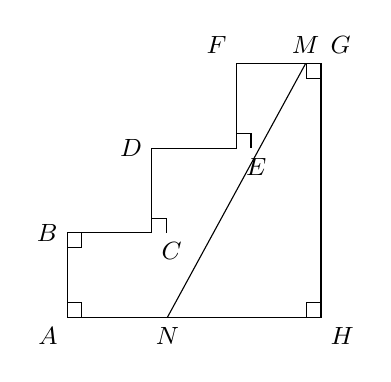
\begin{tikzpicture}[scale=0.62,font=\small]
\coordinate (A) at (0,0); \coordinate (B) at (0,1.732); \coordinate (C) at (1.732,1.732); \coordinate (D) at (1.732,3.464); \coordinate (E) at (3.464,3.464); \coordinate (F) at (3.464,5.196); \coordinate (G) at (5.196,5.196); \coordinate (H) at (5.196,0);
\coordinate (M) at (4.88,5.196); \coordinate (N) at (2.05,0);
\draw (A)--(B)--(C)--(D)--(E)--(F)--(G)--(H)--cycle; \draw (M)--(N);
\draw (0,0.3)--(0.3,0.3)--(0.3,0); \draw (0,1.432)--(0.3,1.432)--(0.3,1.732); \draw (1.732,1.732)+(0,0.3)--(2.032,2.032)--(2.032,1.732);
\draw (3.464,3.464)+(0,0.3)--(3.764,3.764)--(3.764,3.464); \draw (5.196,0.3)--(4.896,0.3)--(4.896,0); \draw (5.196,4.896)--(4.896,4.896)--(4.896,5.196);
\node[below left] at (A) {$A$}; \node[left] at (B) {$B$}; \node[below right] at (C) {$C$}; \node[left] at (D) {$D$}; \node[below right] at (E) {$E$}; \node[above left] at (F) {$F$}; \node[above right] at (G) {$G$}; \node[below right] at (H) {$H$};
\node[above] at (M) {$M$}; \node[below] at (N) {$N$};
\end{tikzpicture}}
\AB{Agar $MN$ kesma sakkizburçak yuzini teng ikkiga bölsa, $MN$ kesma ajratgan şakllar perimetrlari musbat ayirmasini toping: $\left|P_{ABCDEFMN}-P_{MGHN}\right|$.}{Agar $FM=\sqrt2$ bölsa, $MN$ kesma uzunligini toping.}}
\QQ{44}{Şarga eng katta hajmli silindr içki çizilgan. $R$ — şar radiusi, $r$ — silindr asosi radiusi.
\qfig{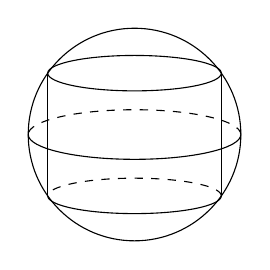
\begin{tikzpicture}[scale=0.9,font=\small]
\draw (0,0) circle (1.5); \draw (-1.5,0) arc (180:360:1.5 and 0.35); \draw[dashed] (1.5,0) arc (0:180:1.5 and 0.35);
\draw (-1.225,-0.866)--(-1.225,0.866); \draw (1.225,-0.866)--(1.225,0.866);
\draw (0,0.866) ellipse (1.225 and 0.25); \draw (-1.225,-0.866) arc (180:360:1.225 and 0.25); \draw[dashed] (1.225,-0.866) arc (0:180:1.225 and 0.25);
\end{tikzpicture}}
\AB{$\dfrac rR$ nisbatni toping.}{Şar hajmining silindr hajmiga nisbatini toping.}}
\QQ{45}{Anvar $24\,000\,000$ söm pulini $A$ va $B$ bankka omonatga qöyadi. $A$ bankdan $1$ yilda oddiy foizda $16\%$ foyda qiladi, $B$ bankdan $1$ yilda oddiy foizda $18\%$ foyda qiladi.
\AB{Agar $A$ va $B$ banklardan $1$ yilda $4\,090\,000$ söm foyda qilgan bölsa, $A$ bankka qança pul qöygan?}{Agar $A$ bankdan bir yilda $2\,240\,000$ söm foyda qilgan bölsa, $B$ bankdan qança foyda köradi?}}
\Javoblar{B A C C C B D A C D C C A C D C B B D C B B B C A B C A C C B A B F C}{%
\OK{36}{$4$}{$\dfrac83$}\OK{37}{$4$}{$6\pi$}\OK{38}{$\dfrac{32\sqrt3}9$}{$\dfrac{4\sqrt7}3$}\OK{39}{$\dfrac23$}{$\dfrac14$}\OK{40}{$8$}{$13{,}5$}%
\OK{41}{$6{,}25$}{$\dfrac12$}\OK{42}{$4$}{$7{,}4$}\OK{43}{$2\sqrt3$}{$\sqrt{35}$}\OK{44}{$\dfrac{\sqrt6}3$}{$\sqrt3$}\OK{45}{$11\,500\,000$}{$1\,800\,000$}}
